\section{The Anonymous Face Tracking Panda}
As previously stated, living with a mental illness can be isolating and the stigma around mental health issues makes people hesitant to seek professional help. The primary purpose of this thesis is to create a functional prototype capable of connecting people with mental health specialists anonymously, while still maintaining patient-therapist empathy.

\subsection{Approach}
A working prototype was developed using Unreal Engine Blueprints (a node-based interface to create gameplay elements), the UE4, Metahumans, and Live Link connected to an iPhone's camera. In the prototype, patients can communicate with mental health specialists via video conferencing anonymously, as patient's smartphone functions as a virtual camera that allows the mental health practitioner to see the patient's facial expressions in real-time via a virtual avatar.

Using an Apple device with the TrueDepth sensor and the Live Link Face app, one can capture numerous facial tracking points by creating a depth map of ones’ face while projecting and analyzing over 30,000 invisible dots, as well as capturing an infrared face image. The data collected by the Apple device and app is delivered to the UE4 environment via a directed internet connection maintained between the user's iPhone/iPad and the Unreal Engine. When data is received by Unreal Engine 4, it is evaluated and turned into VA movements via Live Link Plugin, as shown in Figure \ref{fig:facialExpressions} and Figure \ref{fig:blueprintsData}.

\begin{figure}[!htb]
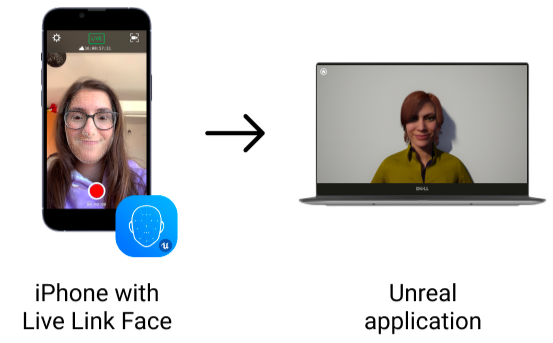
\includegraphics[width=0.7\textwidth]{figures/howItWorks.png}
\centering
\caption{How the facial expressions are captured and represented}
\label{fig:facialExpressions}
\end{figure}

\begin{figure}[!htb]
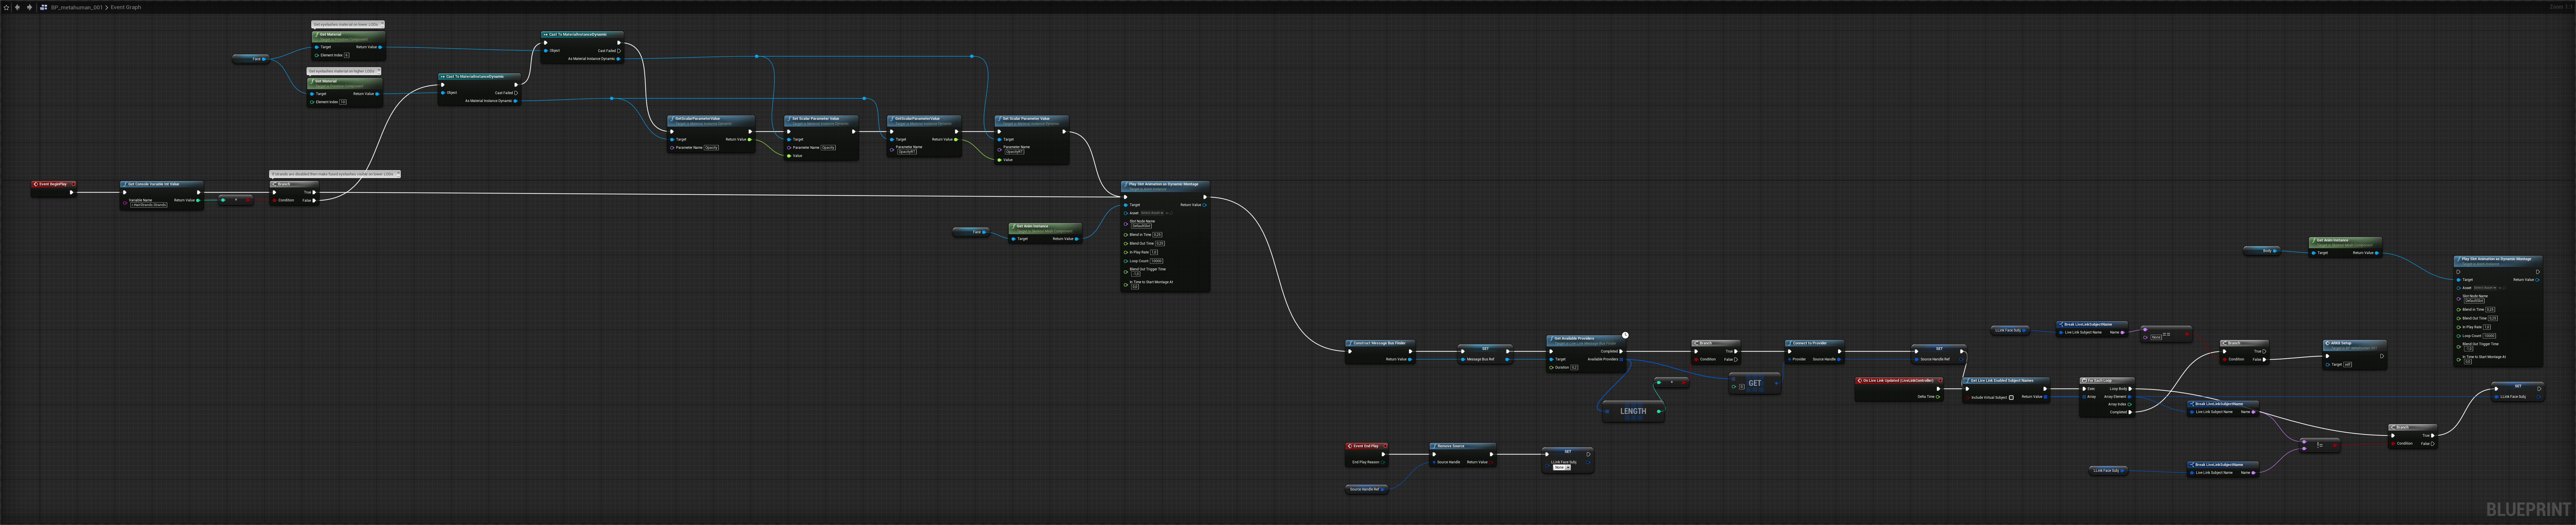
\includegraphics[width=\textwidth]{figures/hereItBegins.png}
\centering
\caption{Blueprints responsible for the connection and stream of data}
\label{fig:blueprintsData}
\end{figure}

The goal of the Live Link Plugin \cite{EPI22} is to provide a unified interface for streaming and consuming animation data into Unreal Engine 4 from one or more external sources, such as Display Data Channel (DDC) tools or Mocap Servers. It's built to be extensible via Unreal Plugins, allowing third parties to create new features without having to make and maintain Engine changes. Live Link can also be used by Motion Capture Systems to stream data into the Engine that can be previewed in real time.

To provide users with options, and thus reach a wider audience, four metahumans (two males and two females, of different ethnicities) were exported from the Metahuman Creator \cite{EPI21}, and the Quixel Bridge application into UE4, where, in order to make the interaction with the prototype easier, a minimalist user interface (Figure \ref{fig:screenshotApp}) was created that allows users to choose their preferred avatar. 

\begin{figure}[!htb]
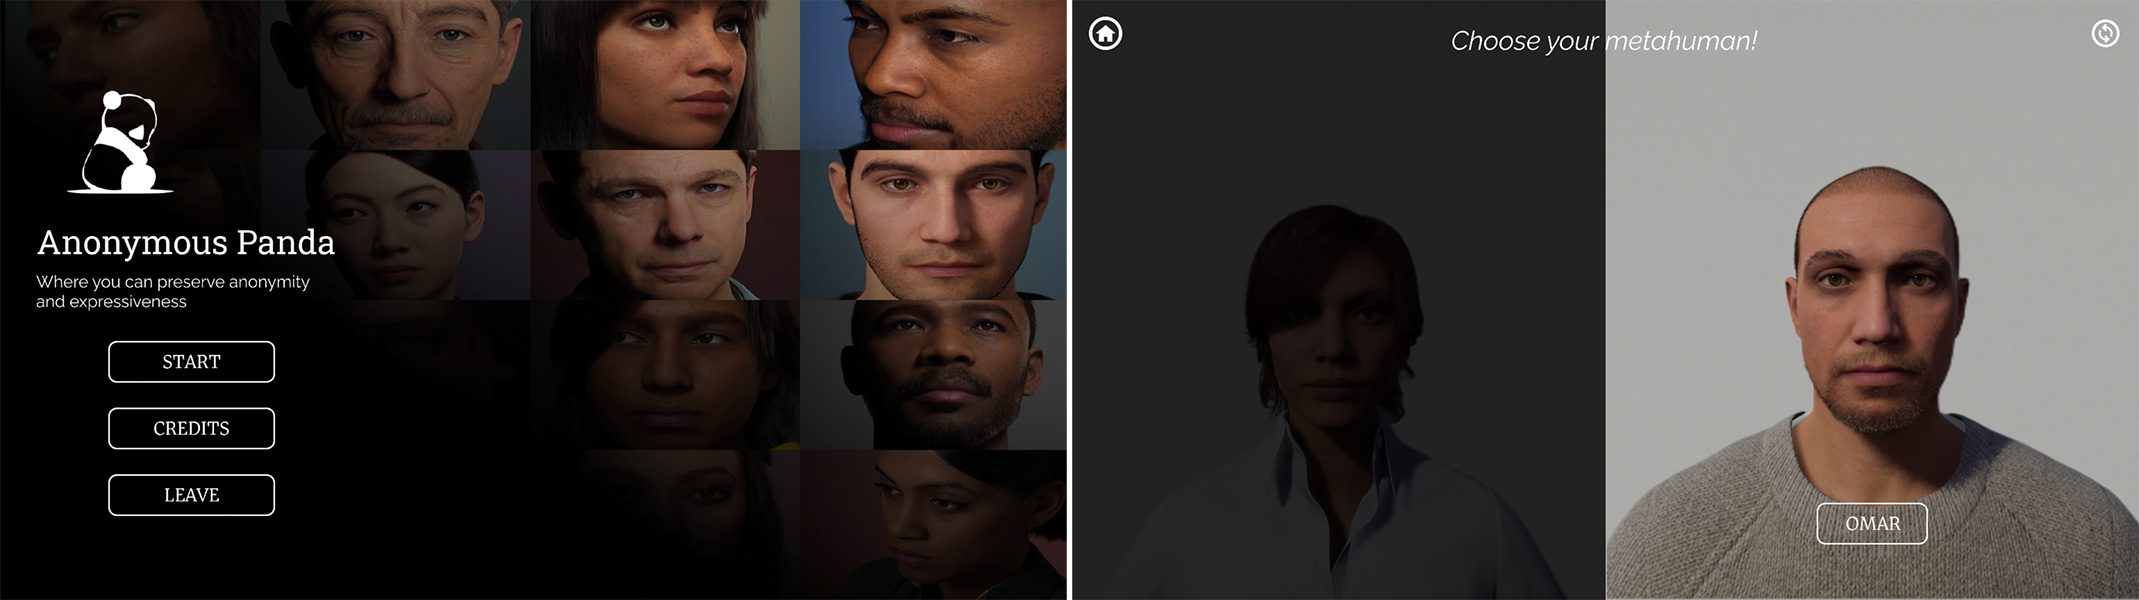
\includegraphics[width=\textwidth]{figures/ui-app.jpg}
\centering
\caption{Screenshots of the Anonymous Panda application}
\label{fig:screenshotApp}
\end{figure}

Although custom metahumans were not employed in this version of the prototype, due to performance and optimization concerns, the chosen metahumans (Figure \ref{fig:metahumans}) were pre-made by Epic Games and available on Quixel Bridge. These concerns were alleviated by using these four metahumans because Epic Games pre-defines export settings and assets compatible with many devices.

\begin{figure}[!htb]
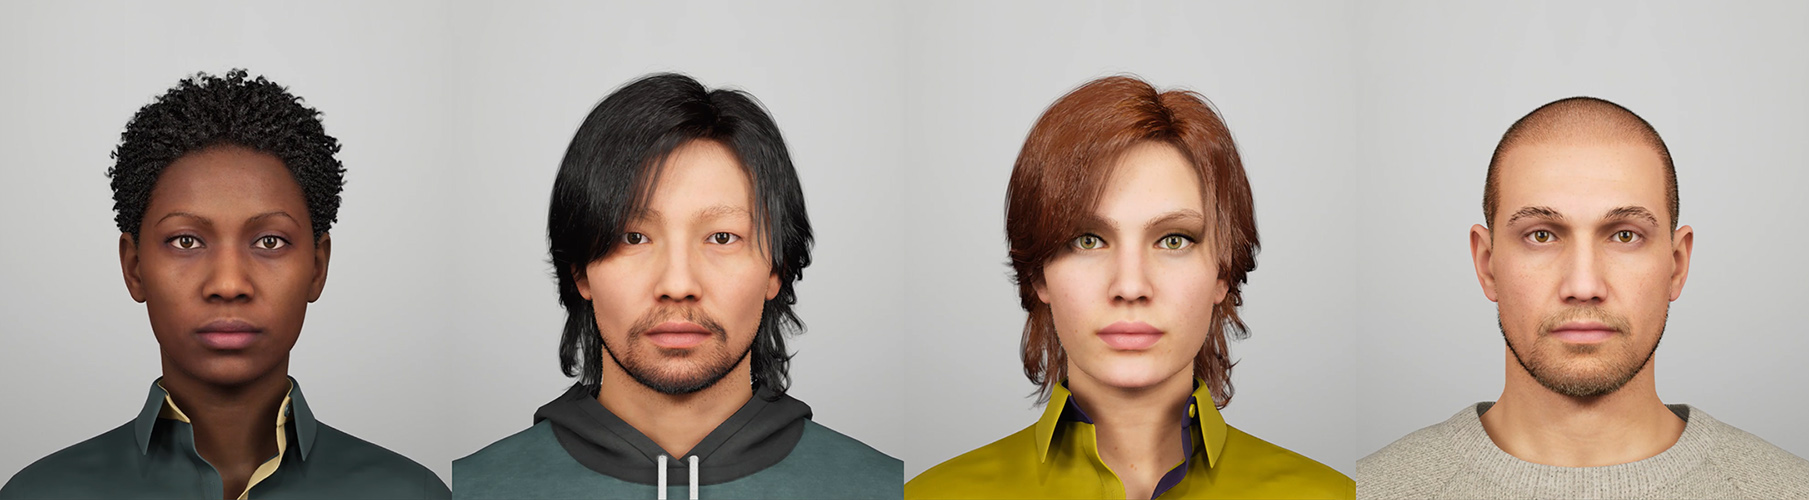
\includegraphics[width=\textwidth]{figures/4metahumans.jpg}
\centering
\caption{The current metahumans used on the prototype}
\label{fig:metahumans}
\end{figure}

As the human face is the primary means of non-verbal communication \cite{MALO20, KUJ03, SAU19}, it is typically used to communicate a person's emotions and mood and to provide visual cues to a person's physical state. Facial expressions are easily distinguished across cultures and automatically perceived so that we can immediately evaluate someone's emotional state. As Figure \ref{fig:metahumanFacialExpressions} makes visible, the facial expression of the VA are perceptible in the current version of the prototype. 

\begin{figure}[!htb]
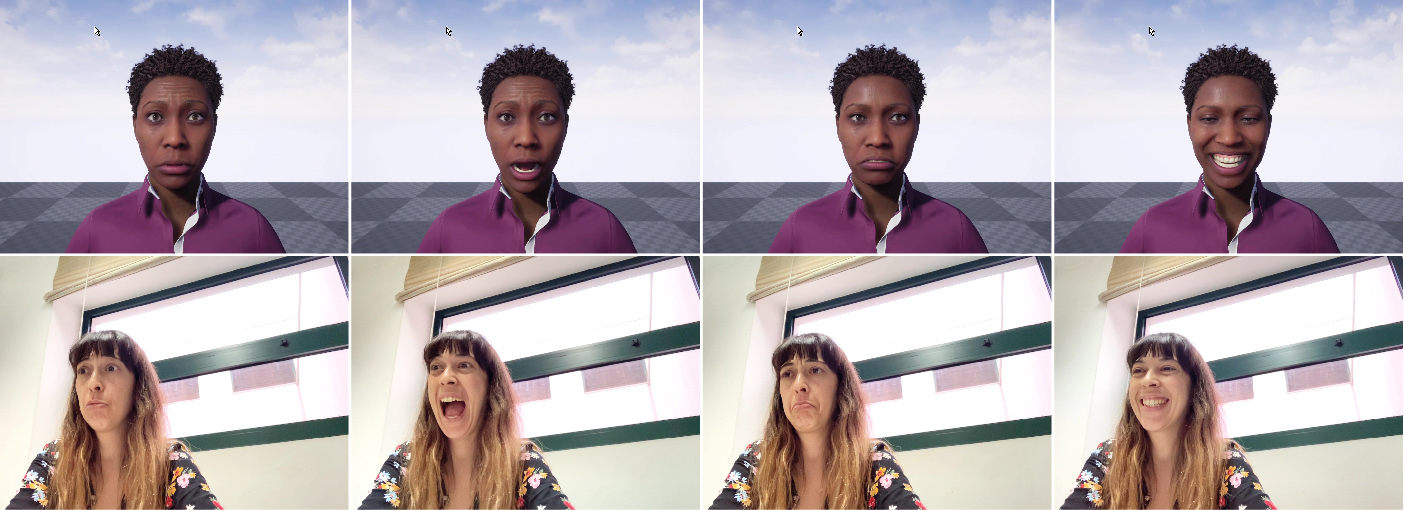
\includegraphics[width=\textwidth]{figures/expressionTest.jpg}
\centering
\caption{Examples of facial expressions and their virtual avatar depiction}
\label{fig:metahumanFacialExpressions}
\end{figure}

However, upon a closer look, even though the avatar could accurately represent the user's facial expressions using the default functions of the live link plugin, a minor flaw in terms of lip positioning was found, particularly when the mouth should be closed or when the user was trying to express a negative emotion (e.g., sadness). To solve this issue, the upper lip values were slightly adjusted (Figure \ref{fig:blueprintAnimation}) before being reconverted to metahuman animation.

\begin{figure}[!htb]
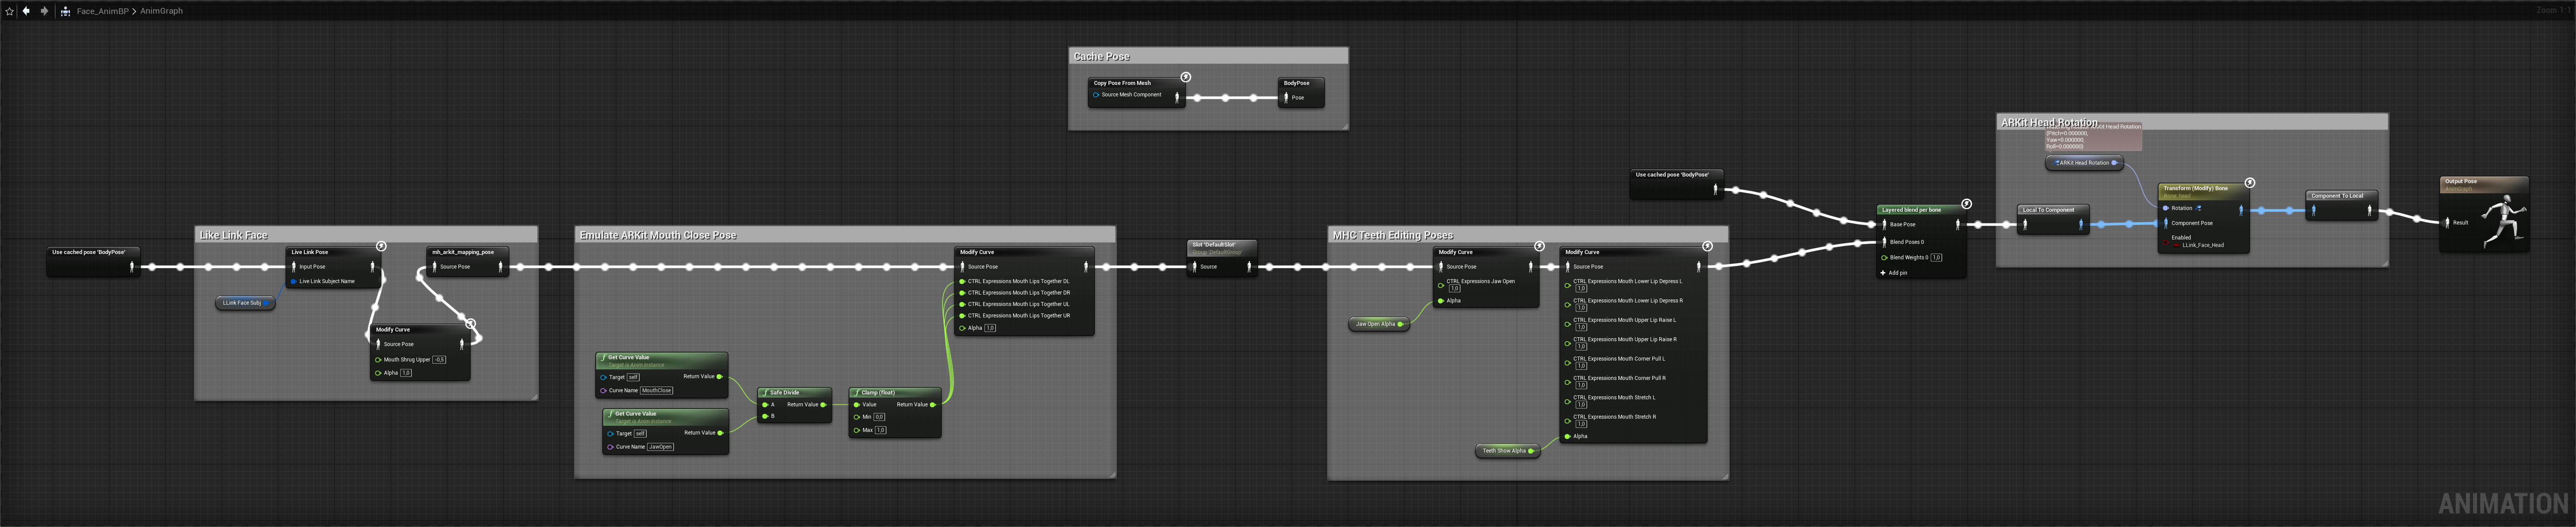
\includegraphics[width=\textwidth]{figures/facialConfig.png}
\centering
\caption{Blueprints responsible for the conversion of data to animation of metahuman}
\label{fig:blueprintAnimation}
\end{figure}

Although one of the foundations of this thesis is patient-therapist communication,  the current prototype requires the user to share only the UE4 application as if it were a webcam, which necessitates the usage of a video conferencing tool as well as OBS Studio Virtual Camera, a live streaming tool (Figure \ref{fig:prototype} and \ref{fig:obs}). Even though this causes a slight delay, it can be used in a video conference.

\begin{figure}[!htb]
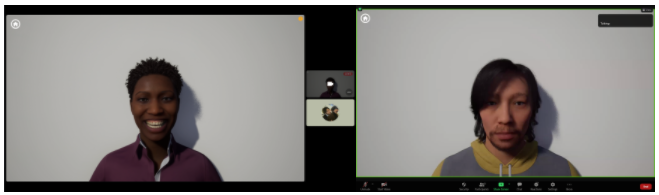
\includegraphics[width=\textwidth]{figures/zoomAndDiscord.PNG}
\centering
\caption{The prototype in use on a call via Discord and Zoom}
\label{fig:prototype}
\end{figure}

\begin{figure}[!htb]
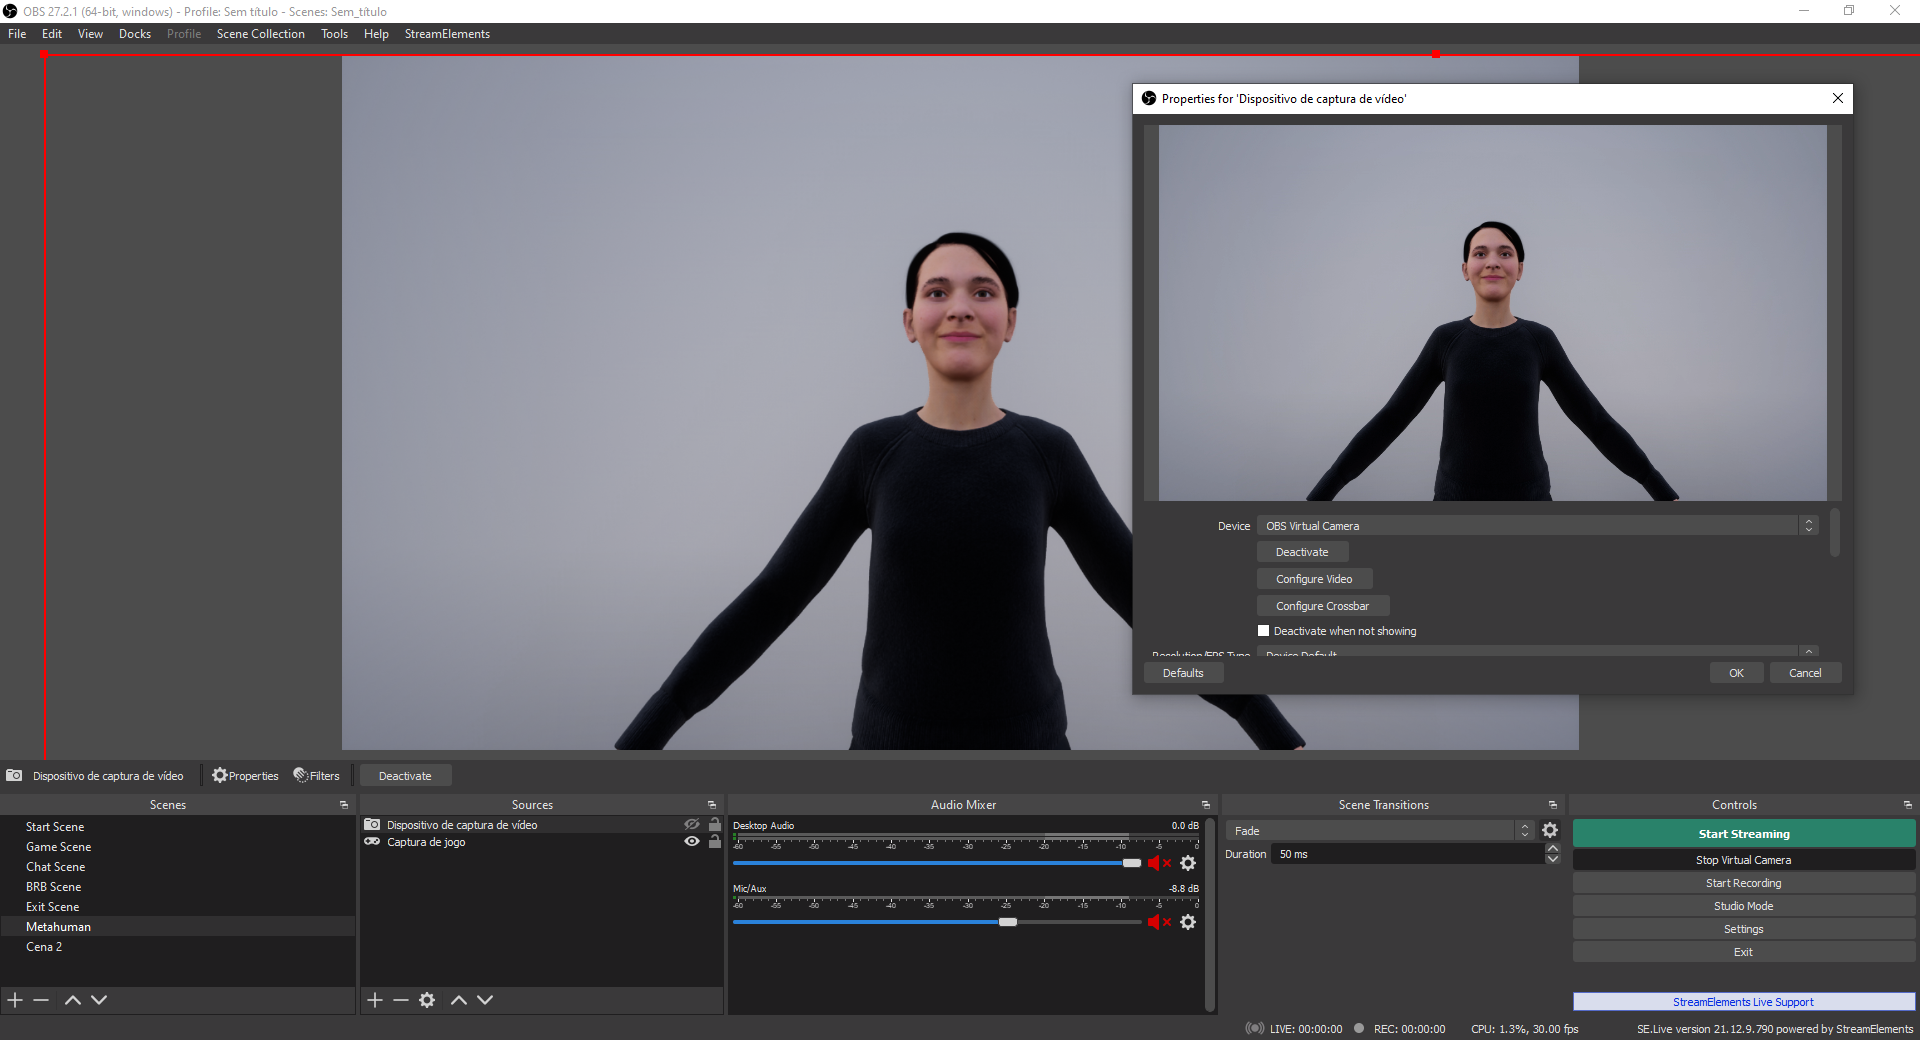
\includegraphics[width=\textwidth]{figures/streamingTool.PNG}
\centering
\caption{Virtual Camera setup on OBS Studio}
\label{fig:obs}
\end{figure}

\subsubsection{Limitations}
One of the thesis's challenges is to use customized models because these models demand a lot of optimization. After all, they are resource-intensive, limiting the patient's expressions from being viewed clearly and fluidly. 

Nonetheless, the creation and use of custom metahumans has already improved thanks to recent contributions from Epic Games. However, because many assets are still in development, the design and use of metahumans are still limited. Meaning, if these assets are excluded, it should be possible to use metahumans other than those pre-defined by Epic Games. Figure \ref{fig:metahumanWarning} shows a warning about using a metahuman with groom elements under development, as well as a warning for only displaying it in Level of Detail (LOD) 0 and 1. The many levels that make up each groom element's LODs set, which includes hair, mustache, beard, eye brows, eye lashes, and vellus (also called peach fuzz), are depicted in Figure \ref{fig:LOD}.

\begin{figure}[!htb]
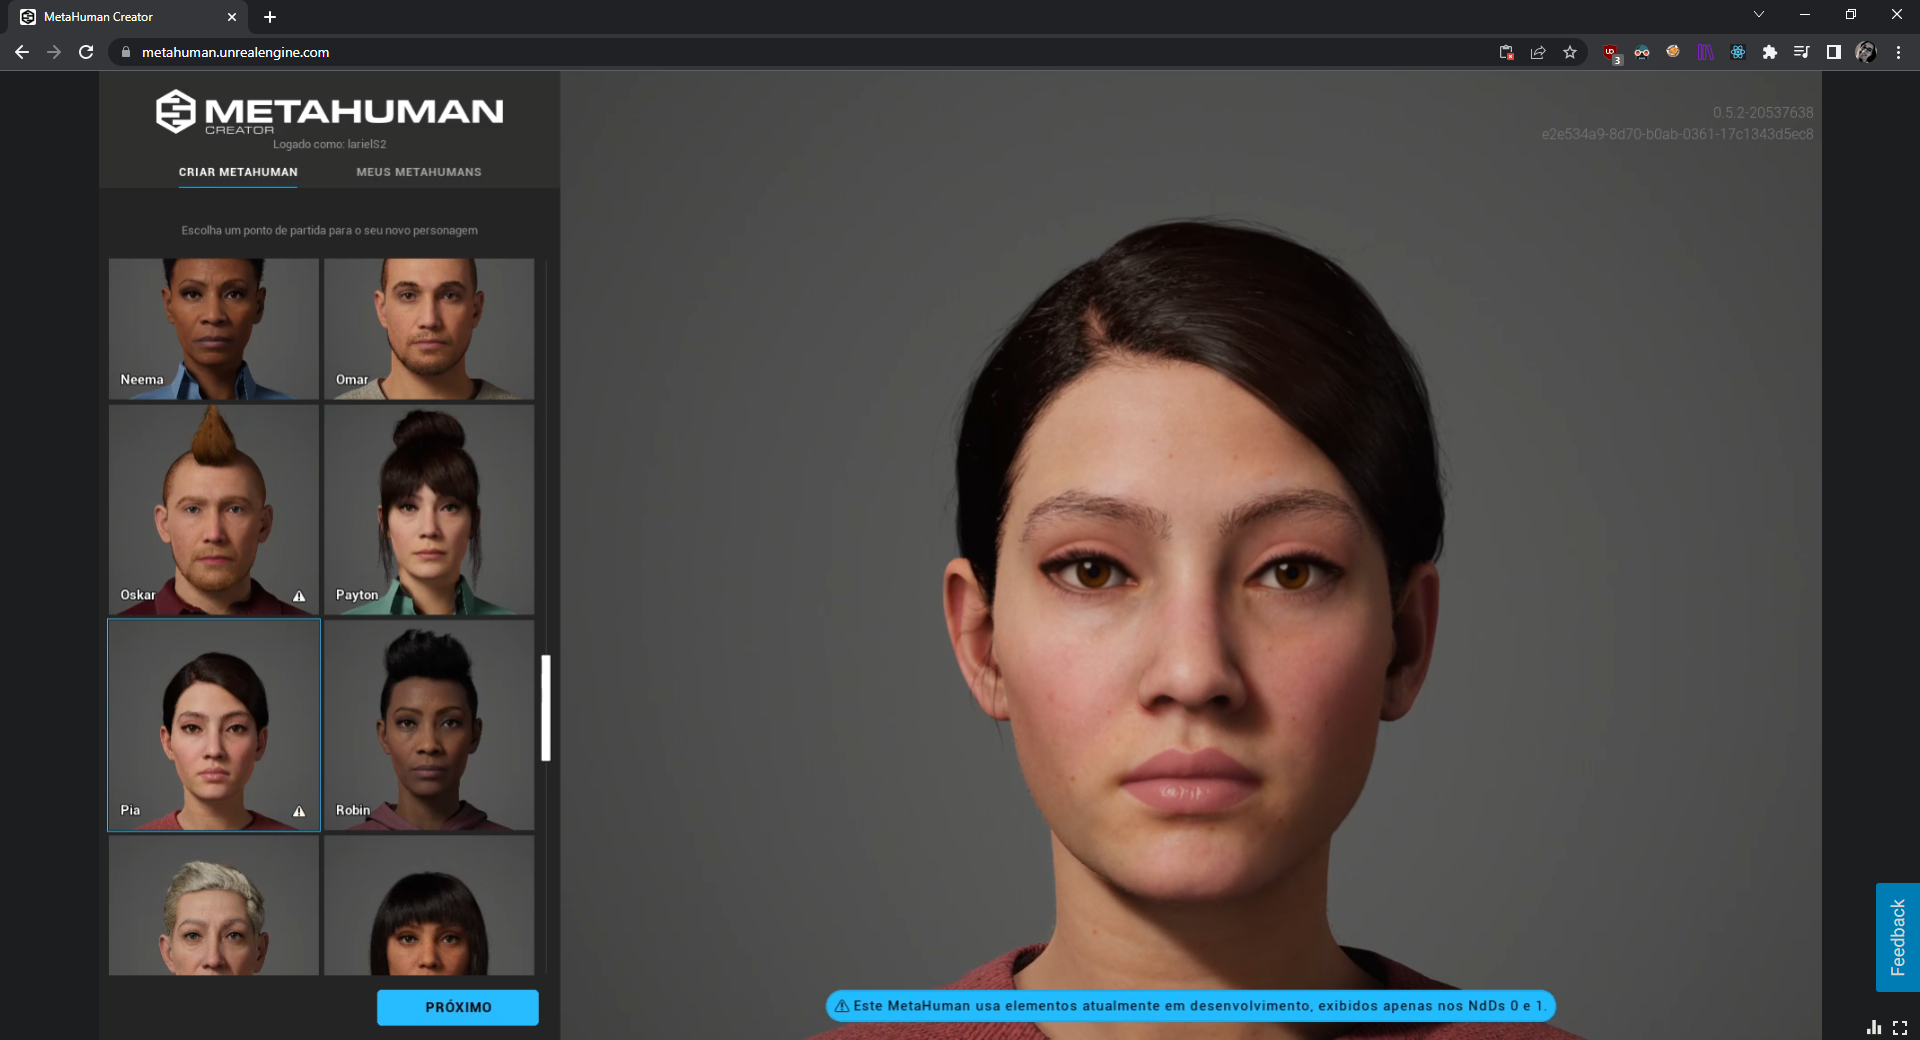
\includegraphics[width=\textwidth]{figures/warningMetahumanCreator.PNG}
\centering
\caption{Metahuman Creator warning for elements under development}
\label{fig:metahumanWarning}
\end{figure}

\begin{figure}[!htb]
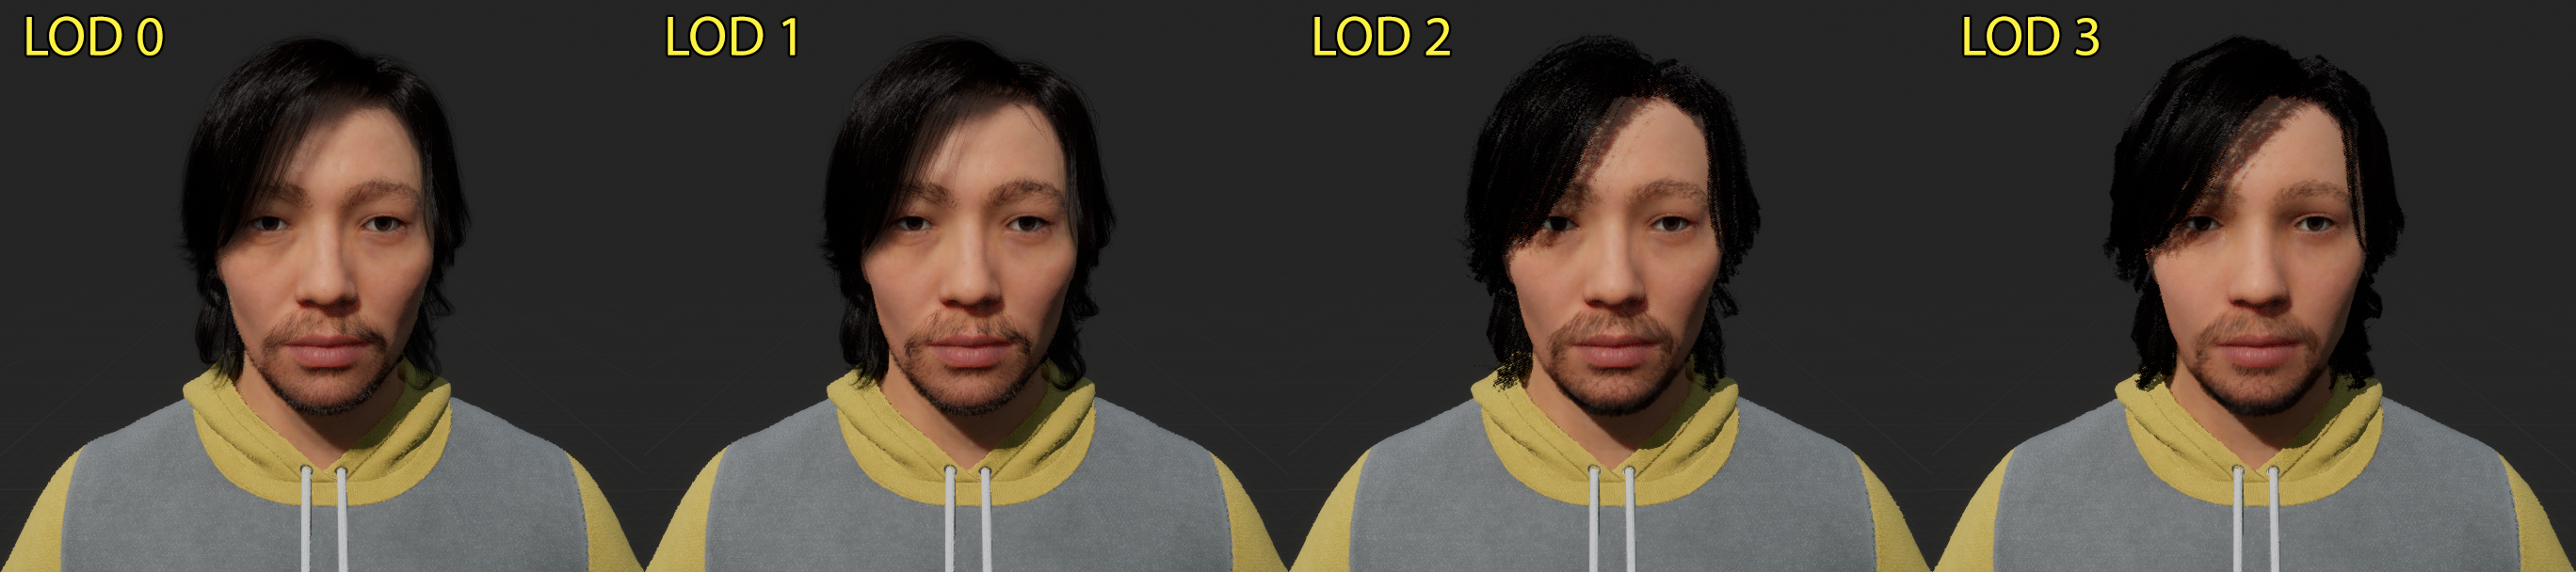
\includegraphics[width=\textwidth]{figures/GroomLODSequence1.PNG}
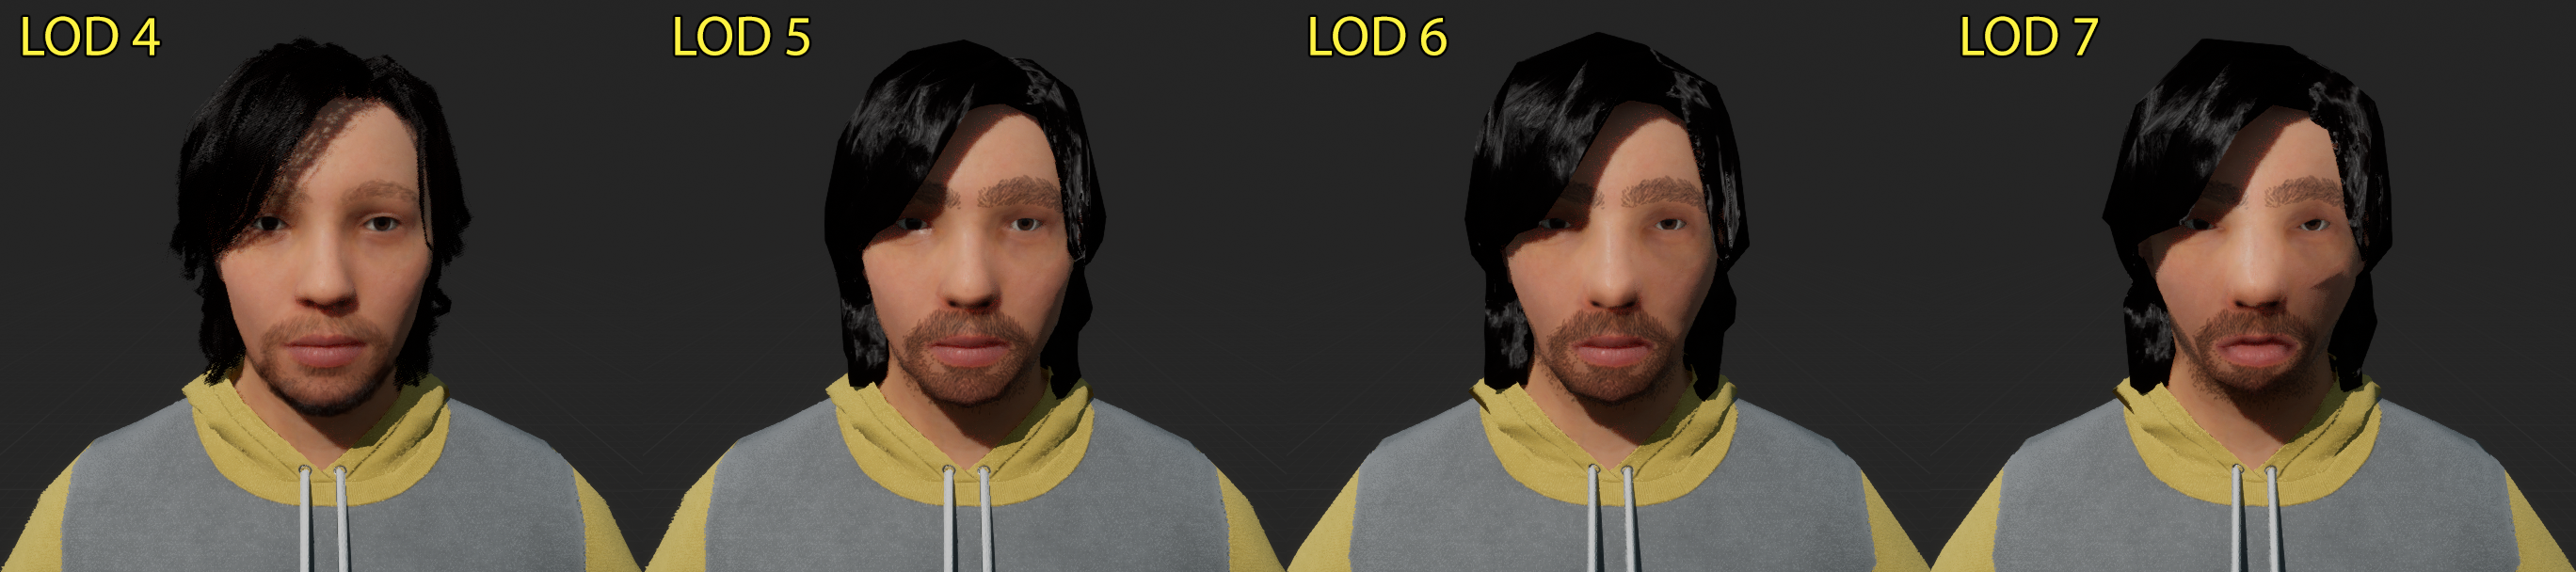
\includegraphics[width=\textwidth]{figures/GroomLODSequence2.PNG}
\centering
\caption{Groom LoD sequence from cinematic (0) to the lowest (7) quality}
\label{fig:LOD}
\end{figure}

Moreover, because this is a resource-intensive application, another difficulty is how people will utilize it. As a result, one of the problems is figuring out how to develop this program to reach everyone who needs it. 

\subsection{Methodology}
To assess the feasibility of the previously described approach and test users' empathy with the metahumans, a controlled experiment that was accepted by the university's Data Protection Officer and authorized by the Ethics Committee, evaluated whether these virtual avatars are able to convey the same emotional depth as a real person (\textbf{RQ\textsubscript{1}}).

We conducted a between-subjects experiment to assess if our independent variable stimulus---which has three levels, metahuman (G\textsubscript{1}), real person (G\textsubscript{2}), and transcript (G\textsubscript{3})---had an effect on participants' cognitive empathy (CE) and affective empathy (AE). We also assessed whether the video had any effect on authenticity and social presence perceived by the participants. Each participant was exposed to the previously mentioned stimulus levels through the following randomly selected tests: a) pre-recorded metahuman, b) pre-recorded person, c) transcript from the previous pre-recorded contents (see Appendix \ref{appendix:story}).

The metahuman was created to match the appearance of the real person (Figure \ref{fig:customMeta}) as close as possible while keeping performance levels high (by using only optimized assets). This was done in order to avoid introducing excessive third-variable bias \cite{ROT19}, and as a way to balance the social presence levels in the metahuman and real person video conditions. The story was chosen from a specific \textit{subreddit} (i.e., an online community where people ask others for advice) based on the amount of \textit{upvotes} (1500) and number of comments (304) received on Reddit, as it provides a metric on user engagement and, therefore, we believe will help elicit empathy in the participants.

\begin{figure}[h!]
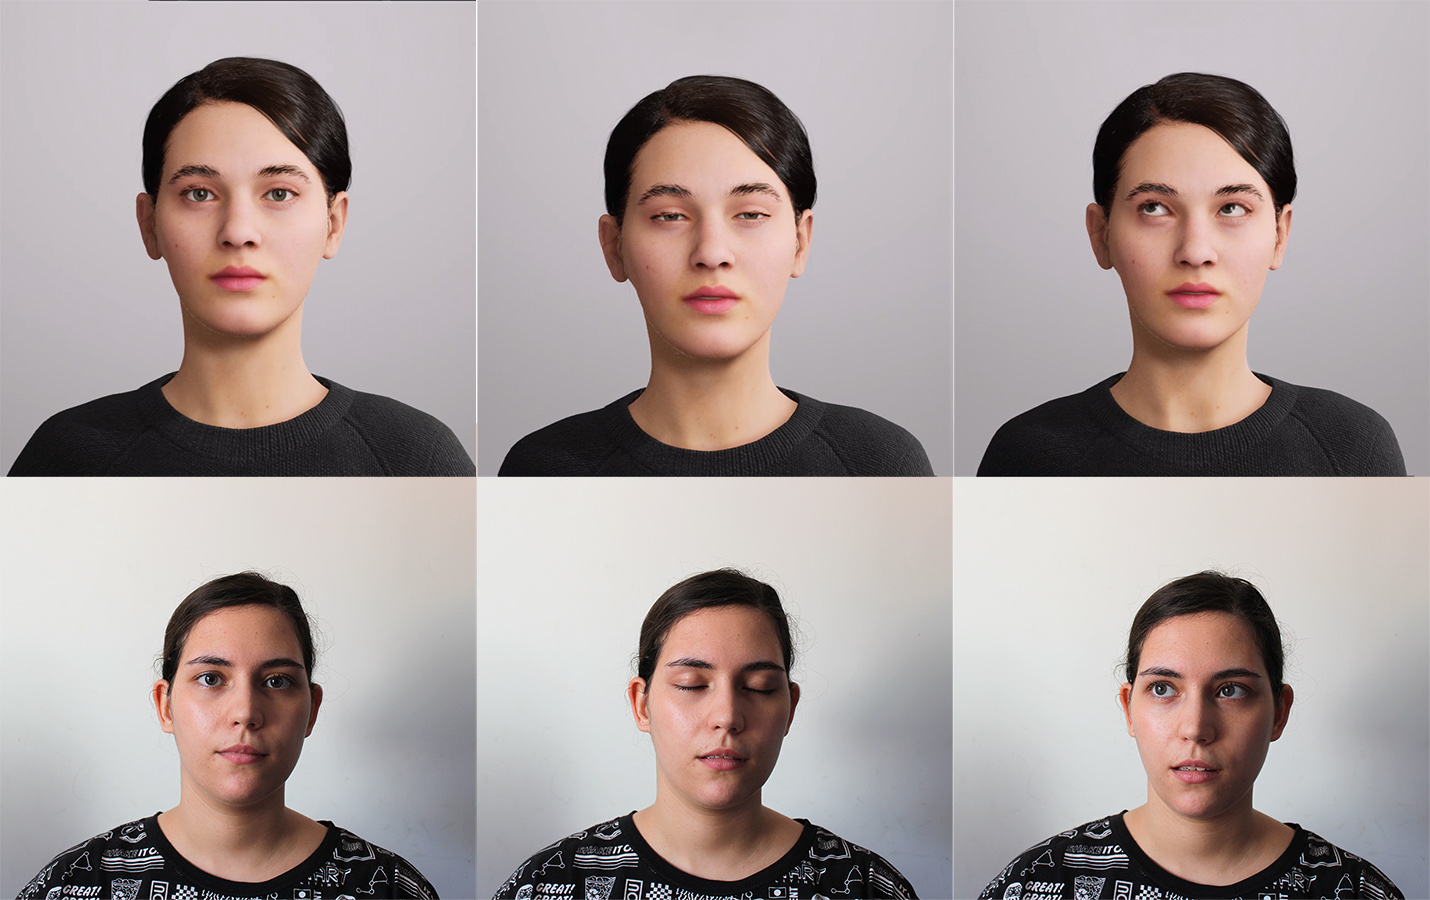
\includegraphics[width=\textwidth]{figures/personavatar.jpg}
\centering
\caption{Different expressions in both the custom metahuman and the actor}
\label{fig:customMeta}
\end{figure}

\subsubsection{Participants}
Participants were required to be at least 18 years old and needed to be college students. They were recruited via email and social media groups, and they were given a general overview of the study's topic. Our final sample consists of 48 college students (25 male, 23 female), aged between 18 and 45 (\textit{M}=23.9, \textit{SD}=5.7).

Those who agreed to participate (\textit{N}=48) were first given an informed consent form. An independent samples design was used for this experiment, where participants were asked to fill out basic demographic questions and a self-assessment questionnaire \cite{SPR03} used to measure their baseline levels of empathy before our stimulus. Then they were randomly allocated to one of the three groups of content (G\textsubscript{1}, G\textsubscript{2}, and G\textsubscript{3}) using an online random redirect tool \cite{FER19} and finally, asked some follow-up questions.

Regarding the score for baseline empathy levels, they can vary from 0 to 64 \cite{SPR09}. Males tend to score in the range of 43.46 to 44.45 on this measure, while females tend to score in the range of 44.62 to 48.93 \cite{SPR09}. In comparison, the mean (\textit{M}) scores in our study for males were 47.08, with a standard deviation (\textit{SD}) of 5.54, whereas for females were 48.65, with a \textit{SD} of 7.49, indicating that our male sample was slightly above average and our female sample was among the average results.

\subsubsection{Procedure}
To recruit participants, an online questionnaire was created and distributed through social media groups, along with emails spread to Madeira University's general student population. Participants (\textit{N}=48) who agreed to participate in the study were first given an informed consent form and properly informed on the study's broad, general topic. 

To prevent revealing the true goal of the experiment and thereby distorting the results, participants were asked to fill out basic demographic questions as well as some general questions about themselves from the Big Five Inventory \cite{JOH91} in addition to the Toronto Empathy Questionnaire \cite{SPR03}. They were then redirected to one of three groups of content (G\textsubscript{1}, G\textsubscript{2}, and G\textsubscript{3}) through \cite{FER19} before being asked to complete a questionnaire meant to assess participants' empathy levels in response to the randomly assigned stimulus, as proposed by  \cite{ROT19, ZIB19}.

As mentioned before, for the pre-stimulus survey (see Appendix \ref{appendix:pre}) we used the Toronto Empathy Questionnaire \cite{SPR03}, which consists of 16 items (e.g., "I become irritated when someone cries", 1=strongly disagree, to 5=strongly agree), as a control variable. Five items from the Big Five Inventory \cite{JOH91} were incorporated into the questionnaire to dispel any suspicions regarding the study's genuine goal.

Regarding the pos-stimulus questionnaire (see Appendix \ref{appendix:videoPost} and \ref{appendix:transcriptPost}), participants were requested to answer questions, related to cognitive and affective empathy  (i.e., our dependent variable), on a seven-point Likert-type scale (1=totally disagree, 7=totally agree), based on the work of Bailenson et al. \cite{BAI03}.

We used four questions to assess the video's perceived authenticity and social presence, presenting the statements: "I feel that the person is watching me and is aware of my presence", "The thought that the person is not a real person crosses my mind often", "The person appears to be conscious and alive to me", and "I perceive the person as being only a computerized image, not as a real person", with the above-noted Likert-type scale.

Then, empathy was tested in both video and transcript groups by using items adapted from the Interpersonal Reactivity Index \cite{DAV83} that deal with  CE and AE. Three items were used to test CE: "I understand what made her get upset", "Her reactions to the situation are understandable", and “I understand her point of view”. Afterwards three items were used to measure AE: "I can relate to her problem", "When I see someone in an unfair situation, I feel frustrated", and “I feel that her emotions are genuine”.

Finally, participants could describe in an open-ended question what made them empathize and/or relate to the person in the video/transcription, as well as what they did not like.

\subsubsection{Hypotheses and Statistical Analyses}
To answer \textbf{RQ\textsubscript{1}} (Can virtual avatars elicit the same emotional response as human-to-human interactions?), we tested if our independent variable stimulus---which has three levels, metahuman (G\textsubscript{1}), real person (G\textsubscript{2}), and transcript (G\textsubscript{3})---had an effect on participants' cognitive and affective empathy. Because the participants' CE and AE are supposed to indicate if the feelings and emotions conveyed via stimulus were understood, it's reasonable to assume that those with greater baseline empathy levels would comprehend the feelings and emotions better.

Therefore, our hypotheses were:

\textbf{\textit{H}\textsubscript{1}} - All stimulus conditions can elicit the same cognitive emotion.

\textbf{\textit{H}\textsubscript{2}} - The metahuman video stimulus can elicit more affective empathy than the real person video stimulus.

\textbf{\textit{H}\textsubscript{3}} - The person video stimulus can elicit more affective empathy than the transcript stimulus.

To test \textbf{\textit{H}\textsubscript{1}}-\textbf{\textit{H}\textsubscript{3}}, we tried to see if the cognitive and affective empathy of each group differed significantly. This required a multivariate analysis method because we look at more than two variables (or factors) and how they might impact our experiment. As a result, we utilized the Kruskal-Wallis H test for ordinal, nonparametric data to see if there were any statistically significant differences in CE and AE between the three conditions.

We also wanted to investigate if the metahuman and real person groups' levels of social presence differed significantly. This required a bivariate analysis method because we only look at two variables (or factors). As a result, we used a Mann-Whitney U test to see if there were any changes in social presence between the metahuman and real-life video situations. Finally, all this data was analyzed in the IBM SPSS statistics software (v.28, 2021), using a statistical significance level of 0.05.

\subsubsection{Results}
To evaluate the differences in cognitive and affective empathy across conditions, we performed a Kruskal-Wallis test. The test showed no statistically significant differences in cognitive (\textit{H(2)}=4.30, \textit{p}=.116) or affective empathy (\textit{H(2)}=.618, \textit{p}=.734) for the three conditions (metahuman, \textit{n}=23; real person, \textit{n}=12; transcript, \textit{n}=14). Table \ref{tab:kwhTest} show the results of the Kruskal-Wallis H test and Figure \ref{fig:kwSamples} show the independent-samples from the Kruskal-Wallis H test.

\begin{table}[!htb]
	\begin{minipage}{0.44\linewidth}
        \begin{tabular*}{\linewidth}{ @{\extracolsep{\fill}} lcc}
        \small & \small CE & \small AE\\
        \hline

        \small Median & \small 6 & \small 5\\
        \small Mean & \small 5.88 & \small 5.25\\
        \small Std. Dev. & \small .981 & \small 1.021\\
        \hline

        \small \textit{H(2)} & \small 4.301 & \small 0.618\\
        \small \textit{p} & \small .116 & \small .734\\
        \hline\\
        \end{tabular*}
        \caption{Results between G\textsubscript{1}, G\textsubscript{2}, and G\textsubscript{3}}
        \label{tab:kwhTest}
	\end{minipage}\hfill
    \begin{minipage}{0.55\linewidth}
        \centering
        \begin{subtable}{0.3\textwidth}
            \centering
            \begin{tabular*}{\linewidth}{ @{\extracolsep{\fill}} lc}
                \small & \small SP \\
                \hline
        
                \small \textit{U} & \small 121.500 \\
                \small \textit{Z} & \small -.192 \\
                \small \textit{p} & \small .848 \\
                \small \textit{r} & \small .004 \\
                \hline\\
            \end{tabular*}
        \end{subtable}
        \begin{subtable}{0.5\textwidth}
            \centering
            \begin{tabular*}{\linewidth}{ @{\extracolsep{\fill}} lcc}
                \small & \small Metahuman & \small Person \\
                \hline
        
                \small Median & \small 5 & \small 5\\
                \small Mean & \small 5.09 & \small 4.91\\
                \small Std. Dev. & \small 1.041 & \small 1,921\\
                \hline\\
            \end{tabular*}
        \end{subtable}
        \caption{Results between G\textsubscript{1} and G\textsubscript{2}}\label{tab:MWTest}
	\end{minipage}\hfill
\end{table}

\begin{table}[!htb]
    \begin{minipage}{\linewidth}
        \centering
        \begin{subfigure}{0.49\textwidth}
            \centering
            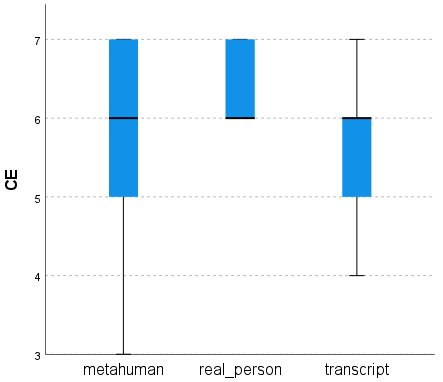
\includegraphics[width=\linewidth]{figures/KW1.png}
            \caption{Cognitive Empathy}
            \label{fig:sub1}
        \end{subfigure}
        \begin{subfigure}{0.49\textwidth}
            \centering
            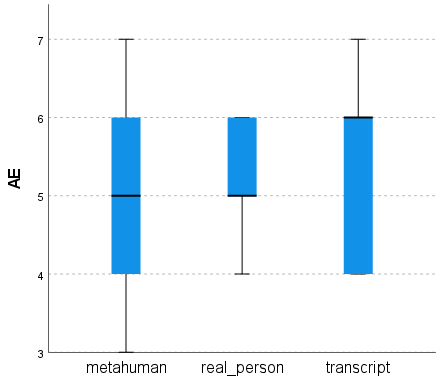
\includegraphics[width=\linewidth]{figures/KW2.png}
            \caption{Affective Empathy}
            \label{fig:sub2}
        \end{subfigure}
        \captionof{figure}{Independent-Samples Kruskal-Wallis}
        \label{fig:kwSamples}
	\end{minipage}
\end{table}

These results support our \textbf{\textit{H\textsubscript{1}}}, namely that cognitive empathy is the same for all conditions. However, no statistically significant differences support our \textbf{\textit{H\textsubscript{2}}}, implying that participants' affective empathy was balanced in both metahuman and real person conditions. The same case was observed with our \textbf{\textit{H\textsubscript{3}}}, where there were no statistically significant differences that could indicate that the person video stimulus elicited higher levels of affective empathy than the transcript stimulus.

\begin{figure}[!htb]
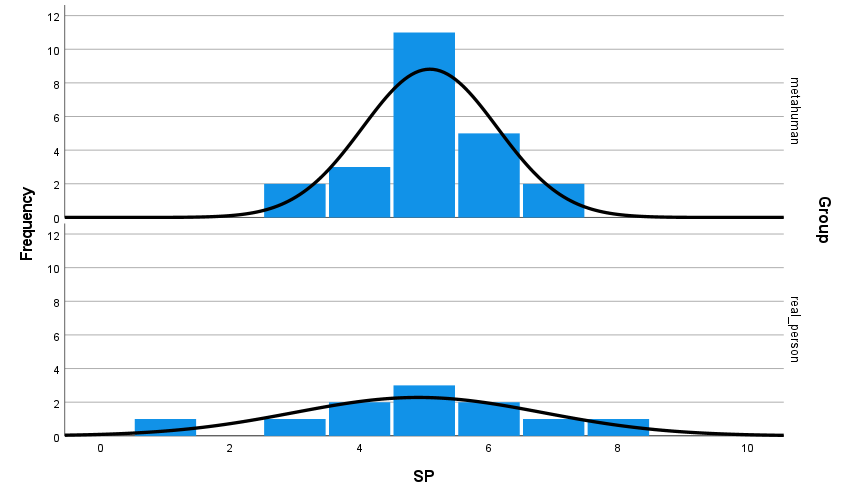
\includegraphics[width=\textwidth]{figures/MWSample.png}
\centering
\caption{Social Presence per group}
\label{fig:MWSample}
\end{figure}

To assess the difference in social presence between the two video conditions, a Mann-Whitney U test was also performed and the results are shown in Table \ref{tab:MWTest}. This test also revealed no significant differences in social presence (\textit{U}=121.500, \textit{Z}=-.192, \textit{p}=.848, \textit{r}=.004) between the metahuman video (\textit{M}=5.09, \textit{SD}=1.041, \textit{n}=23) and the real person video (\textit{M}=4.91, \textit{SD}=1.921, \textit{n}=11). Figure \ref{fig:MWSample} represent the frequency between the social presence levels registered in the metahuman and the real person condition.

\subsubsection{Discussion}
In the present work, we analyzed how metahumans were able to convey the same emotional depth as a real person (\textbf{RQ\textsubscript{1}}). We wanted to see if our independent variable stimulus---metahuman (G\textsubscript{1}), real person (G\textsubscript{2}), and transcript (G\textsubscript{3})---had any influence on participants' cognitive and affective empathy.

We found that all our conditions could elicit participants' cognitive empathy, which means that they were able to put themselves on the side of the storyteller and see the storyteller perspective. However, we can display cognitive empathy without feeling sympathy for it because all we have to do is put ourselves in someone else's shoes to experience it. Recent research by Fernandez and Zahavi on the ideas of emotional and cognitive empathy shows that none of these concepts adequately describe the most fundamental type of empathy. In their study, which looks into the role of empathy in nursing work, the authors claim that cognitive empathy enables nurses to comprehend their patients while keeping a professional distance and objectivity \cite{FER20}. This supports what we previously suggested, which is that one does not have to feel sympathy for others in order to comprehend them. 
This means that, while the results confirm our \textbf{\textit{H\textsubscript{1}}}, they could be easily skewed because we used a self-reported questionnaire, therefore there's a chance that individuals gave invalid answers \cite{DEM15}.

Regarding our \textbf{\textit{H\textsubscript{2}}}, we did not find significant differences in the level of affective empathy elicited by the avatar versus the real human. As a result, regardless of whether it was conveyed through the avatar or the real person, a self-disclosing story elicited similar levels of AE. Our findings support previous research on similar perceptions of avatars and human stimuli \cite{ALI15, ROT19}. We discovered a positive effect of authenticity on both cognitive and affective empathy, which supports our \textbf{RQ\textsubscript{1}} that realistic avatars, in this case metahumans, may convey the same emotional depth as a real person. This may be interpreted as an indication that high authenticity enables the willingness to accept a different perspective and predict the internal emotional states of others. Another, more limiting interpretation is that the audio for each condition was kept consistent, and so voice was a strong carrier for the perception of empathy. Additional research needs to be done because we did not examine a limited situation with only voice or with altered voices.

Similarly, no significant differences in affective empathy between the person video stimulus and the transcript were discovered (\textbf{\textit{H\textsubscript{3}}}). As a result, participants' levels of AE were similar whether they heard the narrative from the real person or read the transcript themselves. This could be related to the narrative itself, as it was chosen from a \textit{subreddit} where people ask others for advice and it was a story that everyone can relate to as it is a typical everyday situation that could happen to any of us. Another interpretation might be based on how the person in the video portrayed themselves and how well it reflected the story's emotions because the participants were able to understand that person's circumstances and feelings, just as those who merely read the narrative did.

Finally, we evaluate the difference in social presence between the two video settings (metahuman and real person) in order to validate our \textbf{RQ\textsubscript{1}} that realistic avatars may transmit the same emotional depth as a real person. Our findings revealed no significant differences in social presence between the metahuman video and the real person video. However, these results suggest that our avatars' level of realism can perform just like a real person would and thus be used as a webcam in video conference systems.